\documentclass[journal]{IEEEtran}

\usepackage{cite, graphicx}
\usepackage[usenames,dvipsnames]{xcolor}

% *** GRAPHICS RELATED PACKAGES ***
%
\ifCLASSINFOpdf
  % \usepackage[pdftex]{graphicx}
  % declare the path(s) where your graphic files are
  % \graphicspath{{../pdf/}{../jpeg/}}
  % and their extensions so you won't have to specify these with
  % every instance of \includegraphics
  % \DeclareGraphicsExtensions{.pdf,.jpeg,.png}
\else
  % or other class option (dvipsone, dvipdf, if not using dvips). graphicx
  % will default to the driver specified in the system graphics.cfg if no
  % driver is specified.
  % \usepackage[dvips]{graphicx}
  % declare the path(s) where your graphic files are
  % \graphicspath{{../eps/}}
  % and their extensions so you won't have to specify these with
  % every instance of \includegraphics
  % \DeclareGraphicsExtensions{.eps}
\fi

\usepackage[cmex10]{amsmath}
%\usepackage{algorithmic}
\usepackage{algorithm}
\usepackage{algorithmicx}
\usepackage{algpseudocode}
\usepackage{listings}
\usepackage{tikz}

\usepackage{array,multirow,graphicx}
\usepackage{xspace}
\usepackage{amssymb, stmaryrd, algorithm, mathrsfs}
\usepackage{mdwmath}
\usepackage{mdwtab}
\usepackage{eqparbox}
\usepackage{lipsum}
%\usepackage[tight,footnotesize]{subfigure}
%\usepackage[caption=false]{caption}
%\usepackage[font=footnotesize]{subfig}
%\usepackage[caption=false,font=footnotesize]{subfig}

%\usepackage{fixltx2e}

\usepackage{stfloats}
%\usepackage{url}\newcommand{\urlb}[1]{{\color{blue}\url{#1}}}
\usepackage{color}
\usepackage{hyperref}
\hypersetup{
  colorlinks   = true, %Colours links instead of ugly boxes
  urlcolor     = blue, %Colour for external hyperlinks
  linkcolor    = blue, %Colour of internal links
  citecolor   = red %Colour of citations
}

\usepackage{amssymb}\newcommand{\todonote}[1]{\footnote{\color{red}TODO: #1}\marginpar[\color{red}\hfill$\blacktriangleright$]{\color{red}$\blacktriangleleft$\hfill}}

\newcommand{\csp}{\textsc{CSP}\xspace}
\newcommand{\cop}{\textsc{COP}\xspace}
\newcommand{\ghost}{\textsc{GHOST}\xspace}
\newcommand{\ie}{\textit{i.e.}}

\newcommand{\modelcsp}[4]%
{ \begin{trivlist}
  \item[]%
    \textbf{CSP model for #1}:\\
    \textit{Variables:} #2\\
    \textit{Domain:} #3\\
    \textit{Constraints:} #4
  \end{trivlist}%
}

\newcommand{\modelcop}[5]%
{ \begin{trivlist}
  \item[]%
    \textbf{COP model for #1}:\\
    \textit{Variables:} #2\\
    \textit{Domain:} #3\\
    \textit{Constraints:} #4
    \textit{Objectives:} #5
  \end{trivlist}%
}

% *** Do not adjust lengths that control margins, column widths, etc. ***
% *** Do not use packages that alter fonts (such as pslatex).         ***
% There should be no need to do such things with IEEEtran.cls V1.6 and later.
% (Unless specifically asked to do so by the journal or conference you plan
% to submit to, of course. )

% correct bad hyphenation here
\hyphenation{op-tical net-works semi-conduc-tor}

\begin{document}

% \lstset{
%   language=[ISO]C++,
%   basicstyle=\footnotesize,
%   keywordstyle=\color{red}\bfseries,
%   commentstyle=\color{violet}\textit,
%   stringstyle=\color{blue}\ttfamily
% }%,labelstyle=\tiny}


%
% paper title
% can use linebreaks \\ within to get better formatting as desired
\title{\ghost: A Combinatorial Optimization Framework for Real-Time Problems}
%
%
% author names and IEEE memberships
% note positions of commas and nonbreaking spaces ( ~ ) LaTeX will not break
% a structure at a ~ so this keeps an author's name from being broken across
% two lines.
% use \thanks{} to gain access to the first footnote area
% a separate \thanks must be used for each paragraph as LaTeX2e's \thanks
% was not built to handle multiple paragraphs
%

% \author{FirstName~LastName,~\IEEEmembership{Member,~IEEE,}
%         Jim~Raynor,~\IEEEmembership{Fellow,~RR,}
%         and~Sarah~Kerrigan,~\IEEEmembership{Life~Fellow,~ZS}% <-this % stops a space
% \thanks{FirstName~LastName is with the Department of Names
% GA, 30332 USA e-mail: (see http://www.michaelshell.org/contact.html).}% <-this % stops a space
% \thanks{J. Raynor and S. Kerrigane are with the Romeo\&Juliet Inc.}% <-this % stops a space
% \thanks{Manuscript received April 19, 2499; revised January 11, 2500.}}

\author{Florian~Richoux\thanks{Florian~Richoux is with the LINA of the Universit{\'e} de Nantes, France, and the JFLI of the University of Tokyo, Japan.},
        Alberto~Uriarte\thanks{Alberto  Uriarte is  with the  Computer
          Science Department  at Drexel University,  Philadelphia, PA,
          USA.},
        Jean-Fran{\c  c}ois~Baffier\thanks{Jean-Fran{\c  c}ois~Baffier
          is with the National Institute of Informatics, Japan.}}



% note the % following the last \IEEEmembership and also \thanks - 
% these prevent an unwanted space from occurring between the last author name
% and the end of the author line. i.e., if you had this:
% 
% \author{....lastname \thanks{...} \thanks{...} }
%                     ^------------^------------^----Do not want these spaces!
%
% a space would be appended to the last name and could cause every name on that
% line to be shifted left slightly. This is one of those "LaTeX things". For
% instance, "\textbf{A} \textbf{B}" will typeset as "A B" not "AB". To get
% "AB" then you have to do: "\textbf{A}\textbf{B}"
% \thanks is no different in this regard, so shield the last } of each \thanks
% that ends a line with a % and do not let a space in before the next \thanks.
% Spaces after \IEEEmembership other than the last one are OK (and needed) as
% you are supposed to have spaces between the names. For what it is worth,
% this is a minor point as most people would not even notice if the said evil
% space somehow managed to creep in.

% The paper headers
\markboth{TCIAIG ~Vol.~X, No.~Y, Month~Year}%
{??? \MakeLowercase{\textit{et al.}}: \ghost: A Combinatorial Optimization Framework for Real-Time Problems}

\maketitle

\begin{abstract}
  This paper  presents \ghost, a combinatorial  optimization framework that
  a Real-Time Strategy (RTS) AI developer can use  to model and solve any problem encoded
  as a constraint satisfaction/optimization problem.  We show a way to
  model   three  different  StarCraft (the RTS game used as a testbed)  problems  as a   constraint
  satisfaction/optimization  problem, and  test our framework on  them.  Each  problem  belongs  to  a
  specific level  of abstraction (the  target
  selection as \emph{reactive control} problem, the wall-in as a \emph{tactics} problem and the build order planning
  as a \emph{strategy} problem). In our experiments, \ghost shows  very good results computed  within some tens
  of milliseconds.
\end{abstract}

\begin{IEEEkeywords}
Game AI, Real-Time, Strategy, RTS, StarCraft, CSP, COP, Solver,
Optimization, Combinatorics.
\end{IEEEkeywords}

% For peer review papers, you can put extra information on the cover
% page as needed:
% \ifCLASSOPTIONpeerreview
% \begin{center} \bfseries EDICS Category: 3-BBND \end{center}
% \fi
%
% For peerreview papers, this IEEEtran command inserts a page break and
% creates the second title. It will be ignored for other modes.
\IEEEpeerreviewmaketitle

\section{Introduction}\label{sec:intro}

\IEEEPARstart {O}{ne} can see games  as a simplification of the world:
The playground  is smaller, rules  are easier and less  numerous, thus
possibilities  are more  limited. However,  games are  rich enough  to
propose complex and dynamic environments where it remains difficult for a
computer  to make  predictions,  have a  global  understanding of  the
current situation  and then make  a decision. This is  specially true
when  information is  incomplete, forcing  the computer  to infer  the
global state of the game from  pieces of information. This is the case
with Real-Time Strategy  games (RTS), where a Clausewitz's  fog of war
hides  the opponent's  moves.  Thus,  RTS games  are very  suitable to
design  Artificial  Intelligence (AI) techniques  that  could  be  applied
afterward in other domains.

Many AI techniques are used in RTS games. Without making an exhaustive
list,  we  can  cite   reinforcement  learning,  case-base  reasoning,
Bayesian programming, goal-driven autonomy,  potential fields, or influence maps. We
recommend  the  reader to  look  at  surveys from  Onta{\~n}{\'o}n  et
al.~\cite{OntanonSURCM13} and Robertson and Watson~\cite{RobertsonW14}
to have a complete overview of AI techniques in RTS games.

However,  there  are  few  works  in  RTS  game  AI  using  constraint
programming    techniques,    in   particular    through    constraint
satisfaction/optimization problem  (\csp/\cop) models.   Among others,
branch and bound algorithms have been  used to optimize build order in
Churchill and Buro~\cite{ChurchillB11}.   Genetic algorithms have been
used off-line to  optimize build order, with  multiple objectives, and
have  been   analyzed  in   Kuchem  et  al.~\cite{KuchemPR13}.   And  a
population-based   algorithm  has   been   used  for   multi-objective
procedural    aesthetic   map    generation    in   Lara-Cabrera    et
al.~\cite{LaraCF14}.    Still,   \csp/\cop    offers   a   convenient,
homogeneous framework able to model a huge number of combinatorial and
optimization problems,  and proposes  a various  set of  algorithms to
solve them.

\csp/\cop is widely used in  AI to solve problems
like  path-finding, scheduling,  and  logistics.  Unlike  mathematical
programming, \csp/\cop  algorithms are  usually not designed  to solve
one  specific problem  but are  general, able  to manage  any problem
modeled in that framework. Besides the generality, it is also easy and
intuitive  to model  a problem  with a  \csp/\cop.  Altogether,  these
bring  ideal  conditions  to   design  and  develop  a  user-friendly,
easy-to-extend, general solvers.


\subsection{RTS problem families}

Onta{\~n}{\'o}n et  al. propose in~\cite{OntanonSURCM13}  to decompose
RTS  problems  into  three  families,  according  to  their  level  of
abstraction. From  the higher to  the lower level, these  families are
(extracted from~\cite{OntanonSURCM13}):
%--------------
\begin{itemize}
\item {\bf  Strategy}: corresponds  to the high-level  decision making
  process.   This is  the highest  level of  abstraction for  the game
  comprehension.   Finding an  efficient strategy  or counter-strategy
  against a given opponent is key  in RTS games. It concerns the whole
  set of units and buildings a player owns.
\item {\bf Tactics}:  are the implementation of  the current strategy.
  It implies army and building  positioning, movements, timing, and so
  on. Tactics concerns a group of units.
\item {\bf Reactive  control}: is the implementation  of tactics. This
  consists   in  moving,   targeting,  firing,   fleeing,  hit-and-run
  techniques  (also  knows  as ``kiting'')  during  battle.   Reactive
  control focuses on a specific unit.
\end{itemize}
%--------------
Problems from different families  usually involve different algorithms
to solve them.  In  this paper, we will model one  problem for each of
these three families,  and use our framework \ghost to  solve them, without
any modifications  of its inner  solver. Only  problem models  will, of
course, differ.

\subsection{StarCraft: Brood War}

StarCraft:  Brood War  is the  expansion of  the game  StarCraft, both
released in 1998  by Blizzard Entertainment.  It is an  RTS game where
three  different  races (Terran, Protoss and Zerg)  can be played,
giving an  asymmetric but perfectly  well balanced strategy  game.  In
this paper,  the term  ``StarCraft'' will actually  refer to  the game
plus its expansion StarCraft: Brood War.

A player  has to  gather two  types of resources (minerals and  gas) in
order   to  construct   buildings. Those buildings are necessary to produce  units, to  upgrade
properties such as damage points or armor, and to unlock technologies
and special abilities. Producing units cost resources depend on their properties (hit points, damage points, or size).

The game  is played on  a rectangular map,  discretized into two  types of
tiles: \emph{walkable}  tiles, composed of  $8 \times  8$ pixels and  \emph{buildable} tiles
composed of $4  \times 4$ walkable tiles, \ie, $32  \times 32$ pixels. The
difference  between these  two types  of tiles  would be  explained in
Section~\ref{sec:wall},  while introducing  the wall-in  problem. Like
every RTS game, the map is covered by a fog of war, only dissipated
around our own units/buildings. This means that one cannot know at any
time the full state of the game.   Also, the player has to deal with a
supply capacity, limiting the number of  units he can have. The player
can increase  it by constructing  the right building or  producing the
right unit, according to the race.

StarCraft has  been a world wide  success, and it is still  the most sold
RTS game of the history with nearly 10 millions of copies distributed\footnote{\url{http://www.msnbc.msn.com/id/18925251/}}. It has
been  and  still is  particularly  popular  in  South Korea,  where  a
StarCraft league has  been specially created for  the game, organizing
televised  tournaments between  sponsored players  and teams.   Korean
professional players, or pro-gamers, are  reputed to be among the best
StarCraft pro-gamers in the world.

The flow of time in StarCraft is complex:  The game has 7  speed modes from
``slowest'' to ``fastest'' where ``normal'' corresponds to the regular
 frame rate  (15 logic frames per  second). This is why when we will  write about in-game time, all along this
paper, we will refer to the term \emph{StarCraft unit time} rather than
seconds, to not make any confusions with proper seconds. In the fastest
mode, one logical game  frame takes 42~ms. In StarCraft AI  competitions, it is
necessary  for bots  to not  make  computations longer  than 55~ms  per
frame, in which  case the bot automatically looses the  game after 200
frames exceeding 55~ms.

\subsection{Goals and summary}

The research  presented in this  paper is  an extension of  Richoux et
al.~\cite{RichouxUO14}, where  the problem to  make a wall at  a given
chokepoint (a narrow passage) in StarCraft  has been  modeled  and solved  thanks to  an
ad-hoc algorithm.

The goal of this paper is double:
\begin{itemize}
\item  To present  to  the RTS  AI community  our  frameworl \ghost,  its
  architecture,  how  to model  different  problems  with it  and  the
  results we obtained.
\item To show that constraint  programming can be successfully used in
  RTS AI, at any level of abstraction.
\end{itemize}

The paper is organized as follows: In Section~\ref{sec:ghost}, we give
a     short     introduction     or     reminder     on     constraint
satisfaction/optimization problems,  how they model problems  and what
kind  of algorithms  exists to  solve them.   Then, we  present \ghost
architecture, what  user is aimed, how  to use it to  solve an already
encoded  problem  and how  to  write  your  own problems  via  \ghost.
Sections~\ref{sec:target},~\ref{sec:wall}     and~\ref{sec:bo}    give
details about three  different problem, each one from a  specific level of
abstraction (from  the lower to  the higher: Reactive  Control, Tactics
and Strategy), how  we model them into a \csp/\cop  and what results
we obtain by applying  \ghost. Section~\ref{sec:SOTA} matches \ghost
with  state-of-the-art   constraint  solvers.   Finally,   this  paper
concludes with future work.

\section{\ghost:   A  General   meta-Heuristic  Optimization   Solving
  Tool}\label{sec:ghost}
\subsection{A brief introduction to \csp / \cop}

Constraint  Satisfaction Problems  (\csp) and  Constraint Optimization
Problems  (\cop)   are  two  close  formalisms   intensively  used  in
Artificial  Intelligence  to   solve  combinatorial  and  optimization
problems. Constraint  Programming allows an intuitive  and uniform way
to model  problems, as  well as different  general algorithms  are able to
solve any problems modeled by a \csp or a \cop.

The difference between a \csp and a \cop is simple:
%--------------
\begin{itemize}
\item A \csp  models a satisfaction problem, \ie, a  problem where all
  solutions are equivalent; the goal is then to just find one of them,
  if any. For  instance: finding a solution of a  Sudoku grid. Several
  solutions may exist, but finding one is sufficient, and no solutions
  seem better than another one.
\item A \cop models an  optimization problem, where some solutions are
  better than others.  For instance: Several paths may exist from home
  to workplace, but some of them are shorter.
\end{itemize}
%--------------
Formally, a {\bf \csp} is defined by a tuple ($V$, $D$, $C$) such that:
\begin{itemize}
\item $V$ is a set of variables,
\item $D$ is a domain, \ie, a set of values for variables in $V$,
\item $C$ is a set of constraints.
\end{itemize}

A  constraint  $c   \in  C$  can  be  seen  as   a  $k$-ary  predicate
$c:~V^k\rightarrow\{\top,\bot\}$  where  $\top$  can  be  semantically
interpreted by true and $\bot$ by  false. Thus, regarding the value of
the vector $V^k$, we say that $c$ is either {\it satisfied} (equals to
$\top$) or {\it unsatisfied} (equals to $\bot$).

Notice also that $D$ should formally be the set of the domain for each
variable in $V$, thus a set of  set of values. However it is common to
define the same set  of values for all variables of  $V$, thus one can
simplify $D$ to be the set of values each variable in $V$ can take.

A {\bf \cop} a defined by a tuple ($V$, $D$, $C$, $f$) where $V$, $D$ and
$C$ represent the same sets as a \csp, and $f$ is an {\it objective
function} to minimize  or maximize.

Upon a \csp or a \cop, one can build a \csp formula or a \cop formula,
respectively.   A \csp/\cop  formula is  a conjunction  of constraints
from $C$,  each constraint taking their  variables from $V$. We  say a
\csp/\cop formula  is satisfied  if there exists  an assignment  $q: V
\rightarrow  D$   such  each   constraint  of  the   formula  is
satisfied. Considering the  vector $v \in V^n$ of variables  used in a
\csp/\cop formula, a vector $z \in D^n$ such that
$\forall i \in \{1,n\}, z[i] = q(v[i])$ 
is called a {\it configuration}.  Since
\csp/\cop models a specific problem $\mathcal{P}$, a \csp/\cop formula
represents an instance of $\mathcal{P}$.

Roughly speaking,  there exist  two different  kinds of  algorithms to
solve \csp/\cop problems:
%--------------
\begin{itemize}
\item Tree-based  search algorithms,  also called  complete algorithms
  since they completely  explore the search space  of solutions, using
  smart moves  (backtracking, forward  checking, etc) to  localize and
  avoid dead-ends in the search space.
\item Meta-heuristics,  also called incomplete algorithms,  since they
  are based upon local moves to  find optimums, rather than looking at
  the problem as  a whole. In practice, these algorithms  are the only
  viable  methods   to  manage   industrial-size  problems   within  a
  reasonable runtime. On  the other hand, they cannot  prove they have
  found an  optimal solution, neither  they cannot prove there  are no
  solutions to the given problem.
\end{itemize}
%--------------

\ghost uses a  meta-heuristic algorithm,   \emph{Adaptive   Search}   from   Codognet   and
Diaz~\cite{Codognet01}, as the heart of   its   solver. 
The reason we have chosen a meta-heuristics is
simple: To solve combinatorial and optimization problems while playing
a RTS  game, the  solver needs  to be  very fast  to find  a solution,
within some tens  of milliseconds, which is  virtually impossible with
tree-based search algorithms. The reason  we have chosen {\it Adaptive
  Search}, although it is  not a well-known algorithm, its because it is
one of the fastest meta-heuristic algorithm at  the moment, up to our knowledge
(see Caniou et al.~\cite{Caniou14}).

In  the next  sections,  we  will see  that  looking  for the  optimal
solution is not always an  interesting strategy for RTS games. Indeed,
it is sufficient to have a solution ``optimal enough'' in some tens of
milliseconds   rather  than   spending  seconds   to  find   a  global
optimum. Also, the reader has to keep in mind that meta-heuristics are
stochastic methods, then  two runs on the same  problem instance can lead
to  two different  solutions within  the  same runtime.   This is  why
results  in  this  paper  are  the  average  of  10  to  100  repeated
experiments,  regarding the  problem.  These  results with  \ghost are
very good on  all tested problems, and even often  better than results
the reader can find in the current literature.

\subsection{\ghost architecture}

\ghost  is a  C++11 framework\footnote{Source  code available  at
  \href{https://github.com/richoux/GHOST}{github.com/richoux/GHOST}},
under  the  GNU  GPL  v3  license,  designed  to  solve  any  kind  of
RTS-related problems,  as soon as  they are modeled  into a \csp  or a
\cop. Two different users are targeted:
%--------------
\begin{itemize}
\item  The casual  user, who  only  wants to  use \ghost  to solve  an
  already encoded problem,  like the three problems  presented in the next
  sections.   This  user  only  needs to  instantiate  variables,  the
  domain,  constraints and  eventually  an objective  to describe  the
  instance of his problem, and  to call the function \texttt{solve} of
  the inner solver to run the search. This is done in 5 short C++ lines.
\item The developer user, who has  a specific problem not written with
  \ghost yet.  \ghost  has been designed to let  the implementation of
  new problems easy  without changing a single line in  the solver and
  the  existing  code,  and  without expertise  needed  in  Constraint
  Programming.   Also, \ghost inner  solver has  been designed  to have  as few
  parameters  as   possible,  to  avoid  tedious   and  time-consuming
  parameters tuning before obtaining interesting results.
\end{itemize}
%--------------

\ghost is implemented around five main C++ classes: \texttt{Variable},
\texttt{Domain},    \texttt{Constraint},     \texttt{Objective}    and
\texttt{Solver}\footnote{See        \ghost         manual        pages
  (\href{http://richoux.github.io/GHOST/}{richoux.github.io/GHOST/})
  for more  details}. % Interactions between these  classes are depicted
% in Figure~\ref{fig:ghost}.
% %--------------
% \begin{figure}[th]
%   \centering
%   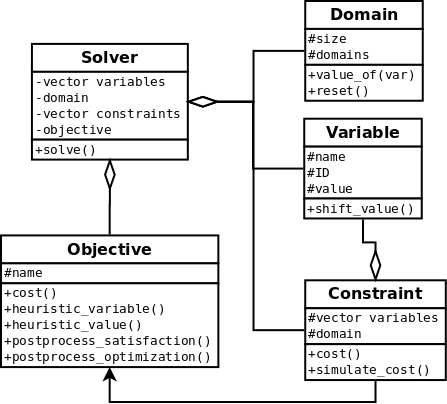
\includegraphics[width=\columnwidth]{figs/ghost_vert.png}
%   %\input{figs/ghost_vert.tex}
%   \caption{A simplified class diagram of \ghost}
%   \label{fig:ghost}
% \end{figure}
%--------------
\begin{figure}[th]
  \centering
  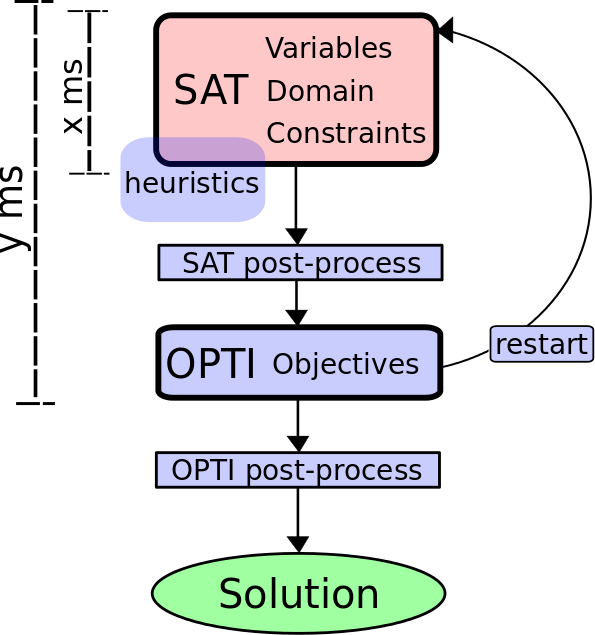
\includegraphics[width=\columnwidth]{figs/archi2.png}
  \caption{\ghost architecture:  In red, the satisfaction  inner loop,
    running  for   $x$  milliseconds   top.   In   blue,  optimization
    mechanisms.    The    whole   process,    excluding   optimization
    post-process, runs under $y$ milliseconds}
  \label{fig:archi}
\end{figure}
%--------------

The  function \texttt{solve}  defined in  \texttt{Solver} follows  the
steps exposed  in Figure~\ref{fig:archi}. It  is composed of  two main
loops: the outer loop for  optimization, containing the inner loop for
satisfaction.      The     satisfaction     part,    in     red     in
Figure~\ref{fig:archi}, only  tries to find a  possible solution among
all configurations, \ie, tries to  find an assignment of each variable
such that all constraints of the \csp are satisfied. It is possible to
call \texttt{Solver::solve} without  defining any objective functions.
In that case,  a default objective is applied,  doing nothing special,
and the solver will output  a solution that satisfied all constraints,
if it finds one.

If an ``real'' objective function  is set, then the optimization part,
in blue  in Figure~\ref{fig:archi}, is  triggered. Even more:  it will
influence  the satisfaction  part (finding  a valid  solution) if  the
objective  implements optional  heuristics to  select the  variable to
change and the value to assign,  if the current configuration is not a
solution.

The  optimization   part  also   applies  two   optional  post-process
optimizations, one on the output of  the satisfaction loop, one on the
final output,  giving the  solution returned by  the solver.   We will
detail  the  purpose  of  such   functions  later,  in  particular  in
Section~\ref{sec:wall}.

The fundamental  thing in  the optimization  part is  the optimization
loop itself. To explain how this  loop works, we have to introduce the
two temporal  parameters in \ghost. The  function \texttt{solve} takes
two parameters: The first one,  mandatory, is the satisfaction timeout
$x$ in  milliseconds.  It means  that, if after  $x$ ms, we  leave the
satisfaction loop, certainly  without a valid solution  since the loop
stops as soon  as it finds a solution. The  second parameter, this time optional
, is the optimization timeout $y$, always in milliseconds. It
corresponds  also  to   the  total  runtime  of   \ghost,  modulo  the
post-process  after  the optimization  loop  (which  is negligible  in
practice and should  be about 100 times smaller than  $y$). If the $y$
parameter is not given, then it is set to 10 times $x$.

Thus, the optimization  loop repeats $n$ times  the satisfaction loop,
and receives  in total $m \leq  n$ valid solutions. After  receiving a
new  solution from  the satisfaction  loop, and  applying an  eventual
satisfaction post-process, it calls  the objective function to compute
the optimization  cost, compares it  with its saved solution  (if any)
and  keeps the  solution with  the lower  cost.  Then  it repeats  the
satisfaction loop  to obtain a new  solution, and so on,  until $y$ ms
are reached.

In some way, \ghost is applying a sort of Monte Carlo sampling. Notice
that this  is not MCTS.   It would  certainly possible to  implement a
MCTS    though   \ghost,    by   twisting    derived   classes    from
\texttt{Variable},     \texttt{Domain},    \texttt{Constraint}     and
\texttt{Objective}, however the authors do not recommend to use \ghost
this  way, since  it should  be more  efficient to  develop a  proper,
ad-hoc MCTS program.

There exists a third and last  parameters in the solver: The length of
the taboo list.  Indeed, {\it Adaptive  Search} contains a taboo list of
explored variables in order to not  revisit the same variable too soon
during the search. The taboo parameter  is then a number expressing how
long  the solver  has  to  wait before  being  allowed  to revisit  an
explored variable. Actually, we  also have implement escape mechanisms
to not make  this taboo list strict,  by allowing the solver  to draw a
taboo   variable   if   there   are   really   no   other   interesting
variables. \ghost's taboo list is thus more like a priority list.

During  our experiments,  we realized  that  the same  value for  this
parameter was  leading to optimal  performances, when set  to $|V|-1$.
It is then a priori not necessary to tune this parameter, however this
remains of course possible to the developer user.

A developer user has to  build his own classes upon \texttt{Variable},
\texttt{Domain},   \texttt{Constraint}   and  \texttt{Objective},   by
inheriting from  them. For  instance, to create  a class  of variables
representing        units,        this        is        done        by
\texttt{class~Unit~:~public~Variable}.   Classes   composed  of  other
classes, like \texttt{Domain} which needs to know on what variables it
will work with, must instantiate  the right templates. Thus, declaring
the   domain   for  the   target   selection   problem  is   done   by
\texttt{class~TargetDomain~:~public~Domain<Unit>}.

Concerning objective  functions, \ghost has been  designed to minimize
their  value.  If  a developer  user  needs to  maximize an  objective
function $f$,  this can be  simply adapted  to \ghost by  defining the
objective  function  $1/f$.   Our  framework is  designed  to  deal  with
mono-objective optimization problem only, thus, one can only choose at
most  one   objective  function  at   the  time  before   running  the
\texttt{solve}  function,  however  the   objective  function  can  be
dynamically changed between two calls of \texttt{solve}. The choice of
designing  a  mono-objective   framework  is  pragmatic:  Multi-objective
solvers are in  general significantly slower, since  dealing with more
complex problems.  Multi-objective solvers  are also more difficult to
implement, which makes harder one goal  of \ghost: To propose a framework
both easy to use and easy to extend by implementing new problems.

In  the next  three sections,  we explain  how we  modeled a  reactive
control  problem, a  tactic  problem  and a  strategy  problem with  a
respective \csp/\cop, and what results we obtained by applying \ghost.
We would like to emphasize that no modifications, no optimizations of the
solver has been  done to manage these different problems.  The core of
the  solver, \ie,  everything  in the  \texttt{Solver} class,  remains
unchanged.  Even  if post-processes  are defined differently  in their
respective \texttt{Objective}  classes, the way they  are included and
called into the solver is rigorously the same.

% \begin{figure*}
%   \begin{lstlisting}
% vector< Unit > variables = { ... }
% vector< UnitEnemy  > enemies  = {  ... }  //specific  to the target selection problem
% TargetSelectionDomain domain( variables.size(), &enemies );
% vector< shared_ptr<TargetSelectionConstraint> > vecConstraints
%       { make_shared<TargetSelectionConstraint>( &vec, &domain ) };
% shared_ptr<TargetSelectionObjective> objective =
%       make_shared<MaxDamage>();
% Solver<Unit, TargetSelectionDomain, TargetSelectionConstraint>
%       solver( &vec, &domain, vecConstraints, objective );
% solver.solve();
% \end{lstlisting}
%   \centering
%   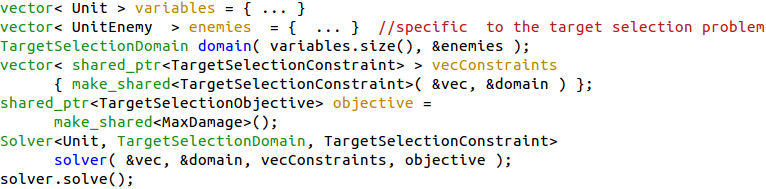
\includegraphics[width=\linewidth]{figs/solve.png}
%   \caption{Example  of  a  casual  use   of  \ghost,  for  the  target
%     selection problem}
%   \label{algo:casual}
% \end{figure*}

\section{Reactive control problem: The target selection}\label{sec:target}

Reactive control problems have been fairly well studied for StarCraft,
with  many different  techniques  applied. We  can  cite Synnaeve  and
Bessi{\`e}re  proposing   in~\cite{SynnaeveB11-b}  a   Bayesian  model
allowing units  to move in  group without  being in each  other's way or
finding the right distance to attack. Uriarte and Onta{\~n}{\'o}n
in~\cite{UriarteO12}  using influence  maps  for  kiting, \ie,  moving
backward while recharging then attacking  forward when one is ready to
shoot.  And Churchill  et  al.  in~\cite{ChurchillSB12,  ChurchillB12}
showing a heuristic search  method making combats outcome predictions.
These two  last papers are also  among the rare ones  dealing with the
target selection problem in StarCraft.

\subsection{Problem statement and model}

The target selection problem is  a classical reactive control problem that
a  player has  to  cope with  it  several times  in  each fight.   Its
satisfaction version  is very easy,  consists in assign  to each
unit of a fighting group a reachable target, \ie, an enemy unit within
our unit range.

In addition, one has also to take  into account a cooldown, that is to
say a fixed number of StarCraft  unit time within a unit recharges and
has to wait  before shooting again.  The cooldown is  the same for all
units of  the same  type.  We  can now  describe the  target selection
problem with the following \csp:
%--------------
\modelcsp{the Target Selection problem}%
{A group of our units.}%
{A group of enemy units.}%
{Each living, ready-to-shoot  unit must aim a living  enemy within its
  range, if any.}

The  target selection  problem is  a frame-by-frame  problem: We  only
consider  the question  ``what  enemy should  I  shoot this  frame?'',
without looking at micro-management moves like kiting.

Usually, RTS games  define specific characteristics to  each unit type
making the target selection more  subtle. Thus in StarCraft, each unit
type  has  a  size  (small,  medium   or  large)  and  a  damage  type
(concussive, normal  or explosive).  Table~\ref{tab:damage}  shows the
damage efficiency  according to  the aimed unit  size and  the shooter
damage type.  For instance, a normal-damage unit will always afflict a
target  with   full  damage,   whatever  the   target  size.    But  a
concussive-damage unit, like a Terran Vulture, will only make 5 damage
points (without counting  upgrade neither armor) against  a large unit
like a Terran Tank, instead of 20 damage points as usual.
%--------------
\begin{table}[!h]
  \caption{Damage efficiency matrix in StarCraft}
  \label{tab:damage}
  \centering
  \begin{tabular}{|c|l|c|c|c|} 
    \cline{3-5}
    \multicolumn{2}{c|}{} & \multicolumn{3}{c|}{Damage type} \\ 
    \multicolumn{2}{c|}{} & \multicolumn{1}{c}{Concussive} & \multicolumn{1}{c}{Normal} & \multicolumn{1}{c|}{Explosive}\\
    \hline
    \multicolumn{1}{|c}{\multirow{3}{*}{\rotatebox[origin=c]{90}{size}}}& {\em Small} & 100\% & 100\% & 50\%\\
    \multicolumn{1}{|c}{} & {\em Medium} & 50\% & 100\% & 75\%\\
    \multicolumn{1}{|c}{} & {\em Large} & 25\% & 100\% & 100\%\\
    \hline
  \end{tabular}
\end{table}
%--------------
Moreover, some  units have a  splash attack, afflicting damage  to the
target's neighbors. In  StarCraft, two splash attack  types exist: The
linear splash, where the  unit can hit a line of  enemies, such as the
Zerg Lurker, and the radial splash  where an attack triggers a circled
shockwave hitting units around the  target within one the three splash
radiuses. The  first radius afflicts  100\% of damage, the  second one
50\% and the  last one 25\%.  Terran Firebat are  special cases mixing
both linear and radial splashes.

Splash  damages combined  with damage  efficiency lead  to interesting
optimization  opportunities.   In  this   work,  we  investigated  two
different objective functions:
%--------------
\begin{itemize}
\item {\bf Max  damage}, where our group tries to  deal as much damage
  as possible within the current frame.
\item {\bf  Max kill},  where our  group tries to  kill as  much enemy
  units as possible within the current frame.
\end{itemize}
%--------------
Notice that these two objective are  more complex that looking for the
maximal  damage  or  the  maximal   dead  enemies  each  unit  can  do
independently. Imagine  a scenario where we  have two units $U_1$  and $U_2$
and two enemies $E_1$  and $E_2$, such that $U_1$ can  afflict 10 damage points
to $E_1$ and 9 to $E_2$, $U_2$ can afflict 8 damage points to $E_1$, but $E_2$ is out
of  range,  and $E_1$  has  5  hit points  (HP)  left.   The best  global
assignment is $U_1$ to  $E_2$ and $U_2$ to $E_1$, even if $U_1$  deals more damage to
$E_1$.

\subsection{\ghost implementation and results}

%Figure~\ref{fig:target}   shows  the   mirror   setup   we  used   for
%experiments. 
Our instance is a mirror setup composed of four lines of units: Line 1
contains 5 marines. Line 2: 2 Goliaths and 2 Vultures. Line 3: 2 Siege
Tanks in tank mode  and 2 Ghosts. Line 4: 1 Siege  Tank in siege mode,
doing splash  damage.  We chose  Terran units  since many of  them are
long-range attack  units and this  makes the target  selection problem
more  interesting.  Also,  we  packed units,  places  them close  each
others, to make significant the Terran Siege Tank's splash damage.
%--------------
% \begin{figure}[!h]
%   \centering
%   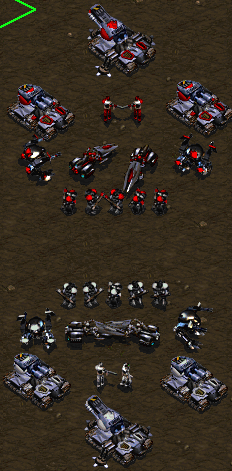
\includegraphics[width=0.8\columnwidth]{figs/target_setup.png}
%   \caption{Mirror  Terran  unit  composition and  placement  used  for
%     experiments. Line 1: 5 marines. Line  2: 2 Goliaths and 2 Vultures
%     (in the middle). Line  3: 2 Siege Tanks in tank  mode and 2 Ghosts
%     (in the middle). Line 4: 1  Siege Tank in siege mode, doing splash
%     damage}
%   \label{fig:target}
% \end{figure}
%--------------
Terran Firebat has not been taking into account in the small simulator
we wrote for testing \ghost on the target selection problem.  We first
planned    to    use   SparCraft~\cite{ChurchillB11,    ChurchillSB12,
  ChurchillB12}, but  we were lacking of  time to learn how  to use it
and combined  it with \ghost. It  was then faster to  develop an quick
ad-hoc simulator (about 200 lines of C++ code).

The simulator is here to emulate a  combat of two unit groups and thus
needs  to  trigger cooldowns,  manage  each  unit HP,  apply  damages and
compute Euclidean  distances between units. Ranges,  damage efficiency
and splash damages are directly managed by \ghost.  It is important to
emphasize that, in this simulator, enemy units are randomly shooting at a
reachable target.

Our simulator does not implement:
%--------------
\begin{itemize}
\item Healing, repair, HP or shield regeneration.
\item Terrain level (high/low ground).
\item Air shots (in StarCraft, there is always a small chance to miss
  the target).
\item Friendly fire.
\item Firebat's unique splash damage.
\end{itemize}
%--------------
\begin{table*}[ht]
  \caption{Average  results over  100 simulations  for both  objective
    functions.%, with  the setup  shown in  Figure~\ref{fig:target}. The
    The first table shows experiments where calls to \ghost lasts for 3~ms,
    and the second table calls lasting for 5~ms}
  \label{tab:target}
  \centering
  \begin{tabular}{|c|l|c|c|c|c|c|c|} 
    \cline{5-8}
    \multicolumn{4}{c|}{}  &   \multicolumn{2}{c|}{\ghost  victory}  &
    \multicolumn{2}{c|}{Opponent victory}\\ 
    \cline{2-8}
    \multicolumn{1}{c|}{}& {\em Objective} &  Win \% & \# Draws & \#  \ghost living units &
    \ghost HP & \# Opponent living units & Opponent HP\\
    \hline
    \multicolumn{1}{|c|}{\multirow{2}{*}{\rotatebox[origin=c]{90}{3~ms}}}&
    {\em Max Damage} & 86.0 & 3 & 2.8 & 153.4 & 1.0 & 37.1\\
    & {\em Max Kill} & 80.0 & 2 & 3.0 & 163.2 & 1.1 & 62.8\\
    \hline
    \hline
    \multicolumn{1}{|c|}{\multirow{2}{*}{\rotatebox[origin=c]{90}{5~ms}}}&
    {\em Max Damage} & 91.0 & 1 & 2.8 & 149.6 & 1.1 & 58.7\\
    & {\em Max Kill} & 82.0 & 3 & 3.0 & 169.5 & 1.0 & 37.2\\
    \hline
  \end{tabular}
\end{table*}
%--------------
We ran 100 simulations for both objective functions until one group is
completely  annihilated,   calling  \ghost  at  each   StarCraft  unit
time. Eventually,  the two groups can  kill one another, leading  to a
draw. We  can then compute \ghost's  win rate, as well  as the average
number of \ghost's  living units at the end of  the simulation and the
average of remaining HP for \ghost  living units when \ghost wins, and
the same  averages when the  opponent wins. For these  experiments, we
first fixed the $x$ satisfaction  timeout and $y$ optimization timeout
parameters respectively  to 1~ms and  3~ms, and we  ran a new  series of
experiments with parameters  $x=2$ and $y=5$.  In~\cite{ChurchillSB12,
  ChurchillB12}, Churchill et al. propose an Alpha-Beta search and run
it  for 5~ms.   This is  why  we have  chosen to  set the  optimization
timeout to  3~ms and 5~ms to  compare our results with  the same timeout
and   with  a   shorter  one.    For  this   problem,  no   particular
post-processing optimizations have been necessary.

Although Churchill et al. method predict a 100\% victory in average in
the different  scenarios they have  tested, the real win  rate in-game
was 84\%.   It is however difficult  to compare their results  to ours
from Table~\ref{tab:target}  for many  reasons: their 84\%  of victory
comes from  in-game experiments against  the built-in AI,  where units
are  moving. Our  simulator,  although realistic  for  damage, do  not
emulate  movements  since  it  is  outside the  scope  of  the  target
selection  problem (\ie,  answering  the question  ``what enemy  units
should I  aim this  frame?''). Plus, the  simulator is  considering an
enemy shooting  randomly, and  the built-in AI  is applying  a smarter
heuristic.

Table~\ref{tab:target}\footnote{All target experiment  results and the
  simulator            can            be           found            at
  \href{https://github.com/richoux/GHOST\_paper/tree/master/xp/target}{github.com/richoux/GHOST\_paper/tree/master/xp/target}}
shows that the Max Damage objective  wins 91\% of the time against the
mirror unit  group shooting  randomly if  we let 5~ms  to \ghost  to do
computations (and 86\% within 3~ms).  The Max Kill objective seems less
efficient with a  win rate of 82\% within 5ms,  (80\% within 3~ms). One
explanation is  that Max Kill  may not be a  heuristic as good  as Max
Damage when enemy  units have their full HP.  It  would be interesting
to cross these two objectives to see if it leads to better results.

For both objectives, we see that \ghost victories are undeniable, with
in average  2.9 remaining units  after the simulation,  whereas losses
are  tight,  with  just one  living  enemy  unit  at  the end  of  the
combat. The average of total remaining  HP is also clearly in favor of
\ghost.

\subsection{Future work}

To go further,  we could implement additional  objective functions for
the target  selection problem, like  minimizing damage waste,  \ie, to
try to  be as close  as 0  HP while killing  an enemy unit  instead of
shooting a  5-HP target with 20  damage points for instance.   Even if
\ghost is  a mono-objective framework,  we could craft new  objectives by
mixing already encoded ones, by simply applying a priority heuristics,
like ``maximize  killings first, and  consider maximizing damage  as a
tiebreaker''.

The current implementation only deals  with Terran ground units for the
target selection problem.   Extending it to all  StarCraft units would
be easy. Finally,  improving the current simulator  or using SparCraft
would make our experiments sharper.

\section{Tactic problem: Wall-in}\label{sec:wall}

Up  to  our  knowledge,  tactic  problems  has  not  been  intensively
investigated for StarCraft.  We can cite however the broadly used BWTA
library implementing  a Voronoi  decomposition to cut  out and  find a
delimitation    between    regions     and    chokepoints    presented
in~\cite{Perkins10}.

However,  the only  works  dealing  with the  wall-in  problem is  the
pioneer paper  from Certicky~\cite{Certicky13} and the  wall-in solver
from Richoux  et al.   in~\cite{RichouxUO14}. As already  written, the
latter provided the basis for the present work.

\subsection{Problem statement and model}

A classical tactic in RTS to defend a base is to make a wall, that is,
to construct buildings side by side in order to close or to narrow the
base entrance. Closing a base gives the player extra-time to prepare a
defense, or  helps him to  hide some  pieces of information  about his
current strategy. Narrowing an entrance creates a bottleneck easier to
defend in  case of  invasion. In  this section we  will focus  only on
walls constructed by buildings,  discarding small narrow passages that
can be closed by small units like workers.

We define  two properties  of buildings: their  {\em build  size}, and
their {\em  real size}.  The  build size is a  pair $(w, h)$  of build
tiles. In  order to  create such  a building, we  need a  rectangle of
buildable tiles  in the map  ($w$ build tiles  in width and  $h$ build
tiles in height). The real size is a pair $(w_p, h_p)$, such that $w_p
\leq 32 \times w$ and $h_p  \leq 32 \times h$, representing the actual
size of  the building  in pixels  once it's  constructed in  the game,
where $32$  is the size  in pixels of a  build tile in  StarCraft. The
real size of a building can then  be smaller than its build size. This
is actually always the case in StarCraft.

This  means that  two buildings  constructed  side by  side are  still
separated by a gap  which may be big enough to  let small units enter,
like Zerglings, Marines  or Zealots. In this paper, we  will call {\it
  significant gap} a gap allowing Zerglings ($16 \times 16$ pixels) to
enter into the base.

The  wall-in  problem has  been  first  modeled  in \csp  by  Certicky
in~\cite{Certicky13}. Then, Richoux et al. proposed a different model,
always  in \csp,  in~\cite{RichouxUO14}.   The work  published in  the
latter has  been \ghost  foundation.  One  can see  \ghost has  a deep
extension and generalization of the solver used in~\cite{RichouxUO14}.

%--------------
\begin{figure}[htb]
  \centering
  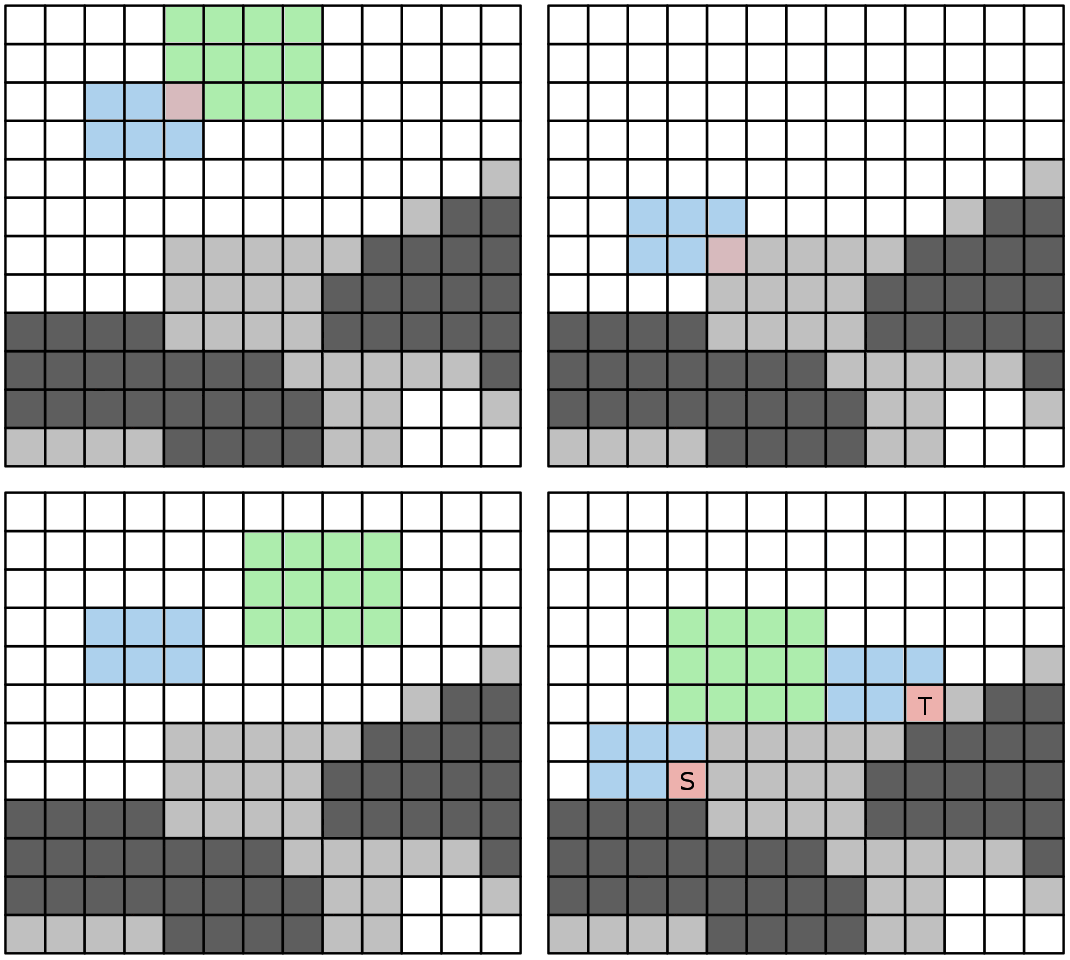
\includegraphics[width=\columnwidth]{figs/all_constraints.png}
  \caption{Constraint    are:    Overlap    (upper-left),    Buildable
    (upper-right),   NoHoles   (bottom-left)  and   StartingTargetTile
    (bottom-right).    Dark  grey   tiles  represent   unwalkable  and
    unbuildable tiles.  Light grey  tiles are walkable but unbuildable
    tiles}
  \label{fig:wall_constraint}
\end{figure}
%--------------

For \ghost, the  model of the wall-in problem is  identical to the one
in~\cite{RichouxUO14}:
%--------------
\modelcsp{the Wall-in problem}%
{Buildings of the player race.}%
{Possible positions around the chokepoint.}%
{Overlap, Buildable, NoHoles and StartingTargetTile.}

Constraints     of      our     models     are      illustrated     in
Figure~\ref{fig:wall_constraint}. They are defined as follows:
%--------------
\begin{itemize}
\item {\bf Overlap}: buildings do not overlap each others.
\item {\bf Buildable}: buildings do not overlap unbuildable tiles.
\item {\bf NoHoles}: no holes of the size of a build tile (or greater)
  in the wall.
\item  {\bf  StartingTargetTile}:  there   are  exactly  one  building
  constructed on a  given starting tile $s$, and one  building (it can
  be the same one) on a given target tile $t$.
\end{itemize}

Actually,  Overlap, Buildable  and NoHoles  are sufficient  to make  a
wall. We added the constraint StartingTargetTile to help the solver to
find how to surround the chokepoint.

\subsection{\ghost implementation and results}

Like for the  target selection problem, we focused on  the Terran race
for  experiments.    The  wall-in  problem  offers   many  interesting
optimization  opportunities.   Therefore,  we have  implemented  three
different objective functions, aiming to minimize:
%--------------
\begin{itemize}
\item {\bf Building}: the number of buildings in the wall,
\item {\bf Gap}: the number of significant gaps in the wall,
\item {\bf  TreeTech}: the required  technology level in the  game (in
  games  like  StarCraft,  some buildings  require  technologies  that
  require resources  to acquire, so  it is interesting to  build walls
  with buildings of low technology).
\end{itemize}
% --------------

To evaluate the  technology level of a wall, we  simply take the depth
in the  technology tree of  the most technological  building composing
the wall. Thus, a Command Center has  a depth 0, a Barracks a depth 1,
a Factory a depth 2, and so on.

This  time, the  satisfaction post-processing  is important  for these
three objective functions, and the optimization post-processing really
helps to improve the Gap and the TreeTech objectives.

The  role of  the  satisfaction post-processing  is  to ``clean''  the
proposed wall, \ie,  to remove all unnecessary buildings  in the valid
solution,  such  that the  resulting  wall  still satisfies  the  four
constraints of the model.

The  optimization  post-processing  used  with the  Gap  and  TreeTech
objectives  tries to  swap each  building  of the  proposed wall  with
another building from  the set of variables $V$, of  the same size and
not already used in the  wall. This simple permutation can drastically
decrease  the number  of significant  gaps between  buildings and  the
technology level required.

% --------------
\begin{table}[ht]
  \caption{Results  over 48  chokepoints  extracted  from 7  StarCraft
    maps. Results  are the  average of 100  runs for  each chokepoint.
    Each calls of \ghost lasts for 150~ms} 
    \label{tab:wall}
    \centering
    \begin{tabular}{|l|c|c|c|}
      \cline{2-4}
      \multicolumn{1}{c|}{}   &    {\em   Satisfaction    run}&   {\em
        Optimization run}& {\em \% solved (opti)} \\
      \hline
      {\em Building} & 4.05 & 2.56 & 98.04\% \\
      {\em Gap} & 1.32 & 0.03 & 97.50\% \\ 
      {\em TreeTech} & 1.99 & 1.35 & 97.54\% \\ 
      \hline
    \end{tabular}  
\end{table}
%--------------
Satisfaction runs in Table~\ref{tab:wall}  are \ghost runs without any
objective functions  and with  a satisfaction  timeout of  160~ms, like
in~\cite{RichouxUO14}  with the  difference that  in Richoux  et al.'s
paper, they  compiled 8 satisfaction runs  of 20~ms each to  have great
chances to find  a valid solution. We measure their  average number of
buildings, significant  gaps and  technology level  in order  to match
them  with   optimization  runs.   Always  following   the  experiment
methodology  of~\cite{RichouxUO14},  optimization  runs  are  slightly
defavored since there global timeout is 10ms shorter than satisfaction
runs, with 150~ms. For optimization  runs, $x$ and $y$ parameters where
fixed   to    20   and   150,    respectively.    We   can    see   in
Table~\ref{tab:wall}\footnote{All wall-in data  and experiment results
  can                   be                  found                   at
  \href{https://github.com/richoux/GHOST\_paper/tree/master/xp/wallin}{github.com/richoux/GHOST\_paper/tree/master/xp/wallin}}
that  optimization  runs  leads   to  real  improvements  compared  to
satisfaction runs. This  is particularly true with  the Gap objective,
where significant  gaps are  almost completely eliminated:  Over 4,800
runs in total, 4,680 walls have been found (97.50\%), and 4527 of them
are perfect walls (\ie, without any significant gaps). In other words,
96.73\% of walls found by \ghost are perfect.

Since  \ghost   code  has  been   improved  compared  to   the  solver
in~\cite{RichouxUO14},  we  obtained   slightly  better  results:  the
percentage  of problems  solved goes  from 95-96\%  to 97-98\%,  walls
decided with  the Building objective  were composed of  2.65 buildings
against 2.56  now, the number  of significant  gaps goes from  0.05 to
0.03 and the technology level from 1.56 to 1.35 currently.
% --------------
\begin{table}[ht]
  \caption{Percentage of solutions found for each map} 
    \label{tab:map}
    \centering
    \begin{tabular}{|c|c|}
      \hline
      Map name & \% solved\\
      \hline
      Python & 100\\
      Heartbreak Ridge & 100\\
      Circuit Breaker & 99\\
      Benzene & 99\\
      Aztec & 97\\
      Andromeda & 96\\
      Fortress & 90\\
      \hline
    \end{tabular}  
\end{table}
% --------------
Table~\ref{tab:map} shows the percentage of walls found in each of the
seven  maps  from where  chokepoints  were  extracted.  These  numbers
correspond  to  pure  satisfaction  runs,  since  they  do  not  defer
significantly for optimization  runs. We can see that  \ghost has more
difficulties to find a wall  for Fortress chokepoints. Actually, it is
failing  from time  to  time on  the same  chokepoint,  where a  valid
solution  can  only  be  achieved  by using  two  $3  \times  2$-sized
buildings.


{\color{blue}
We also performed a comparison between \ghost and the state-of-the-art for the walling problem, in this case the work presented by Certicky~\cite{Certicky13}. First we limited the number of possible buildings to be considered in the wall as the same as Certicky's work (2 Barracks and 4 Supply Depots) and recorded the time to find a solution in two different cases: a small chokepoint (width of 65 pixels) and a big chokepoint (width of {\color{red} 285}). In Table~\ref{tab:wallComparison}\footnote{Comparison experiments can be found at \url{https://bitbucket.org/auriarte/bwta2/src}} we can see the average results of both solvers. The times include the computation needed for setting the solvers parameters, the time to solve the problem, and the time to parse the solution (remember that in the case of Certicky's solution we need to make an external call to Clingo solver). As we can see \ghost is at least 7.8 times faster than Clingo in our experiments.

\begin{table}[ht]
\centering
\caption{Average time over 20 runs to find a solution}
\label{tab:wallComparison}
\begin{tabular}{|r|r|r|r|}
\hline
\multicolumn{1}{|l|}{\begin{tabular}[c]{@{}l@{}}Chokepoint\\ width (pixels)\end{tabular}} & \multicolumn{1}{l|}{\begin{tabular}[c]{@{}l@{}}Buildings\\ needed\end{tabular}} & \multicolumn{1}{l|}{\begin{tabular}[c]{@{}l@{}}GHOST\\ Avg. time (ms)\end{tabular}} & \multicolumn{1}{l|}{\begin{tabular}[c]{@{}l@{}}Clingo\\ Avg. time (ms)\end{tabular}} \\ \hline
65     & 2                                                                             & 46.8                                                                              & 362.8                                                                              \\ \hline
285    & 3                                                                                &                                                                                   &                                                                                    \\ \hline
\end{tabular}
\end{table}
}


\subsection{Future work}

For the wall-in problem, we could add new objective functions to widen
possibilities. For  example, trying to  make a wall by  minimizing the
cost, or the makespan.  This last objective is trickier and related to
the  next  section (it  is  somehow  the  wall-in  + the  build  order
problems).

Most importantly, since  the required runtime to  correctly optimize a
wall is  longer than  a StarCraft frame  duration, we  could implement
\ghost in order  to support computation pauses  and resumes. Actually,
\ghost architecture has been designed by keeping in mind this feature:
The satisfaction  part is executed  in 20~ms,  \ie, it can  be executed
within one StarCraft frame in the fastest mode.  Marking a pause after
each satisfaction loop  and resume \ghost at the next  frame until the
computation ends would not be difficult  to do. This is more discussed
in detail in Section~\ref{sec:conclusion}.

In addition to extend the current  code to manage all StarCraft races,
results in  Table~\ref{tab:map} give us  the feeling that  our wall-in
model  can be  refined again  to reach  a higher  percentage of  found
solutions.


\section{Strategy problem: The build order}\label{sec:bo}

The reader can find an  extensive literature about build order planner
and/or   prediction  for   StarCraft.  Churchill   and  Buro   propose
in~\cite{ChurchillB11} a build order planner  using a branch and bound
technique, Kuchem  et al. analyze  build order tools for  StarCraft II
in~\cite{KuchemPR13},  Cho  et  al.    present  in  ~\cite{ChoKC13}  a
strategy prediction  and build  order adaptation system  learning from
replays and  in~\cite{SynnaeveB11-a} Synnaeve and Bessi{\`e}re  show a
Bayesian model to predict the opponent build order in-game.

\subsection{Problem statement and model}
A build order (BO) planning is a series of actions following a specific
timing, in order to  achieve a goal.  Such a goal  is a combination of
buildings,  units, upgrades  and  researches  produced.  Usually,  the
objective for a  player is to reach a fixed  goal the fastest possible
way. However, alternatives  can also be considered,  like reaching the
goal without sacrificing  the economy, or focusing first  on units in
order to have an army quickly available.

A  BO  planning can  be intuitively  modeled by  a \csp  as a
permutation problem,  where a bijection  maps the set of  variables to
the  domain. Changing  the  value  of one  variable  is then  actually
swapping its value with another variable.

All actions have a (potentially empty) dependency list, \ie, an action
$\alpha$  has a  list of  actions  that are  required before  starting
$\alpha$.   For instance,  to  start the  \textit{Air Weapons  Upgrade
  level 2},  it is required  to have finished the  \textit{Air Weapons
  Upgrade level  1}. Notice  that we can  dive recursively  into these
dependency  lists.  Thus  if someone  aims to  do \textit{Air  Weapons
  Upgrade  level  2}  for  Protoss, it  required  \textit{Air  Weapons
  Upgrade level 1}, which requires itself a \textit{Cybernetics Core},
which requires a \textit{Gateway}.

The \csp model we propose for  the BO planning problem is the
following one:
%--------------
\modelcsp{the Build Order Planning problem}%
{All actions we need to reach our goal.}%
{Order of actions.}%
{Each dependency of an action $\alpha$ must occurs before $\alpha$.}

\subsection{\ghost implementation and results}

We have chosen to  focus on Protoss to test \ghost  on the build order
problem.   The  current  implementation  can  deal  with  any  Protoss
buildings, units, researches and upgrades.

For this  problem, we  have implemented  one objective  function only:
Minimizing the BO makespan.  With  this objective function, we did not
have implemented  a special  satisfaction post-processing, but  we did
for the optimization post-processing. Imagine  the case where the user
asked, among  others, to produce $n$  units of type $U$.  Thus, \ghost
will automatically add, recursively, all  dependencies of $U$ into the
variable set.  Suppose  the unit type $U$ is produced  by the building
of type $B$,  and the user eventually  asked for $m <  n$ buildings of
type $B$.   After having  computed an  optimized BO,  the optimization
post-processing will  retake this solution  and try  to see if  it can
shorten the makespan even more  by constructing more buildings of type
$B$,  to  speed  up  the  production  of  units  of  type  $U$.   This
post-processing optimization  is significantly efficient in  cases the
user ask for a high number $n$ of the same unit $U$, and none or a low
number $m$ of $B$.

Unlike the target selection problem,  we needed this time to integrate
a simulator inside  \ghost to emulate a game (without  combats) and be
able to  compute the  makespan of BOs. Thus,  this simulator
must emulate resources gathering, units producing (including workers),
supply capacity, constructions, etc.  Our simulator will always try to
produce workers  until reaching saturation  (24 workers per  base), as
well as  maintaining supply in  order to never be  ``supply blocked'',
that  is, unable  to  produce a  unit because  we  reached the  supply
capacity limit.

In~\cite{ChurchillB11},  Churchill and  Buro  give  details about  the
simulator they developed for their BO planner.  We first used
the same  settings, but  after matching  \ghost results  against build
order from Korean pro-gamers, we realized that these settings were too
advantageous for the simulator.  We then closely analyzed some replays
from Korean pro-gamers to refine  our simulator settings, listed below
(in StarCraft unit time $t$):
%--------------
\begin{itemize}
\item Time to go build something: 5t (4t in \cite{ChurchillB11})
\item Time to go back  gathering minerals after building something: 4t
  (0 in \cite{ChurchillB11})
\item Time to go from the base  to mineral patches to start mining: 5t
  (0 in \cite{ChurchillB11})
\item  Time for  a worker  to  switch from  mineral  to gas:  5t (0  in
  \cite{ChurchillB11})
\item Mineral gathering  rate: 0.68 mineral per worker per  t (1.07 in
  \cite{ChurchillB11})
\item  Gas  gathering  rate:  1.15  gas per  worker  per  t  (1.66  in
  \cite{ChurchillB11})
\end{itemize}  
%--------------
To be sure these parameters make our simulator realist, we matched its
execution  against the  first  2  minutes of  games  played by  Korean
pro-gamers. Table~\ref{tab:korean}  give an  example of  our simulator
matched against the Protoss Korean pro-gamer Kim "Bisu" Taek Yong. Gas
is not revealed since it remained at 0 for both Bisu and the simulator
during the first 2 minutes. Each time the simulator started to produce
a probe, \ie,  a worker, we write down the  simulator and Bisu mineral
stock and supply situation (used supply over supply capacity). One can
see  that  these two  early  game  are  very  similar, with  a  slight
advantage  to  the simulator  since  its  probe production  is  nearly
perfect.
%--------------
\begin{table*}[ht]
  \caption{Our simulator execution matched  against the pro-gamer Bisu
    during the first two minutes}
  \label{tab:korean}
  \centering
  \begin{tabular}{|c|c|c|c|c|c|} 
    \cline{3-6}
    \multicolumn{2}{c|}{} & \multicolumn{2}{c|}{Simulator in \ghost} & \multicolumn{2}{c|}{Bisu}\\ 
    \hline
    Action (by S(im) or B(isu)) & Time t & \multicolumn{1}{c|}{Mineral} & \multicolumn{1}{c|}{supply (used / capacity)} & \multicolumn{1}{c|}{Mineral} & \multicolumn{1}{c|}{supply (used / capacity)}\\
    \hline
    S starts a probe & 20 & 40.8 & 5/9 & 40 & 5/9\\
    S starts a probe & 44 & 19.7 & 7/9 & 20 & 7/9\\
    S starts a probe & 64 & 46.5 & 8/9 & 50 & 8/9\\
    S starts a pylon & 75 & - & - & - & -\\
    B starts a pylon & 78 & - & - & - & -\\
    S starts a probe & 89 & 1.2 & 9/9 & 12 & 9/9\\
    S starts a probe & 109 & 60.0 & 10/17 & 132 & 9/17\\
    B starts a gateway & 116 & - & - & - & -\\
    S starts a gateway & 125 & - & - & - & -\\
    S starts a probe & 125 & 1.8 & 11/17 & 78 & 9/17\\
    \hline    
  \end{tabular}
\end{table*}
% --------------
\begin{table*}[ht]
  \caption{Average  makespan  of Humans  and  \ghost  BOs  in
    StarCraft unit time over 3647 games. Each calls  of \ghost
    lasts for 30ms}
  \label{tab:bo}
  \centering
  \begin{tabular}{|l|c|c|c|c|} 
    \hline
    \multicolumn{5}{|c|}{Games till 10.000 frames} \\ 
    \hline
    {\em Match-up} & Humans & \ghost & \% solved &
    Gain \\ 
    \hline
    {\em All} & 656.02 & 619.62 & 94.4 & 36.40\\
    {\em PvP} & 651.51 & 608.06 & 95.0 & 43.45\\
    {\em PvT} & 660.50 & 628.17 & 93.9 & 32.33\\
    {\em PvZ} & 649.20 & 609.34 & 95.0 & 39.86\\
    \hline
    \hline
    {\em All pro} & 643.38 & 597.25 & 96.3 & 46.13\\
    \hline
  \end{tabular}
  %\hfill  
  \begin{tabular}{|l|c|c|c|c|} 
    \hline
    \multicolumn{5}{|c|}{Games till 7.800 frames} \\ 
    \hline
    {\em Match-up} & Humans & \ghost & \% solved &
    Gain \\ 
    \hline
    {\em All} & 522.50 & 491.11 & 98.8 & 31.39\\
    {\em PvP} & 516.08 & 485.56 & 99.3 & 30.52\\
    {\em PvT} & 527.66 & 506.65 & 98.3 & 21.01\\
    {\em PvZ} & 515.81 & 458.23 & 99.7 & 57.58\\ 
    \hline
    \hline
    {\em All pro} & 506.38 & 480.88 & 100 & 25.50\\
    \hline
  \end{tabular}  
\end{table*}
%--------------

For  Table~\ref{tab:bo}\footnote{All  build   order  data,  experiment
  results     and     the     simulator    can     be     found     at
  \href{https://github.com/richoux/GHOST\_paper/tree/master/xp/build\_order}{github.com/richoux/GHOST\_paper/tree/master/xp/build\_order}},
\ghost has been  run 10 times on each build  order. We run experiments
on two sets  of build orders: Those extracted from  replays by Gabriel
Synnaeve\footnote{\href{http://emotion.inrialpes.fr/people/synnaeve/TLGGICCUP\_gosu\_reps.7z}{emotion.inrialpes.fr/people/synnaeve/TLGGICCUP\_gosu\_reps.7z}}
and                  refined                  by                  Glen
Robertson\footnote{\href{http://scidrive.uoa.auckland.ac.nz/gameai/scdata/files.txt}{scidrive.uoa.auckland.ac.nz/gameai/scdata/files.txt}},
and those extracted from top Korean pro-gamers.

In total, the first set is  composed of 3647 build orders: 768 Protoss
versus  Protoss, 2043  Protoss versus  Terran and  836 Protoss  versus
Zerg.   Replays where  these  BOs occur  are  coming from  TeamLiquid,
GosuGamers and  ICCup web sites.  Table\ref{tab:bo}  shows that \ghost
outperforms by far human BOs, with  a mean of 36.4 StarCraft unit time
of gain considering 10,000 frames BOs and 31.39 StarCraft unit time of
gain considering 7,800 frames BOs, all match-ups taken together.

We have also  analyzed some few replays of games  played by top Korean
pro-gamers,  \ie, Kim  "Bisu"  Taek  Yong, Doh  "BeSt"  Jae Wook,  Woo
"Violet" Jung Ho, Yang "Cure"  Jung Hyun, all Protoss players, against
Lee  "Flash" Young  Ho (Terran),  Lee  "Jaedong" Jae  Dong (Zerg),  Ma
"sAviOr" Jae Yoon (Zerg) and we  match their build orders with \ghost.
Since we had to manually select those replays, we have only downloaded
6 of them (2 for each  match-up including a Protoss player), giving us
a set of 8 BOs to give to \ghost.

Results against  these pro-gamers are shown  at the very last  line of
Table~\ref{tab:bo}.  One can see that \ghost clearly obtains better BO
than  Protoss Korean  pro-gamers listed  above, with  a gain  of 45.38
StarCraft unit  time for  10,000 frames BOs  and 24.88  StarCraft unit
time  for 7,800  frames BOs.  We  have to  lower the  first result  by
stressing that pro-gamers are often  already engaged in a fight before
10,000 frames and/or are applying outside-the-book strategies, and thus
minimizing the BO makespan may not be their first priority anymore. To
a lesser extent, this is also true with 7,800 frames BOs.

Computation time is  only 20~ms for satisfaction runs and  30~ms for the
(global) optimization run. This means that \ghost can compute a highly
optimized BO  within only one StarCraft frame  at the fastest
speed. In~\cite{ChurchillB11},  Churchill and Buro's branch  and bound
method  is computing  90\%  of the  time BOs  with the  same
makespan as pro-gamers in about 3.735 seconds (for build orders with a
makespan  up to  249s), giving  thus a  CPU time  / makespan  ratio of
1.5\%. Considering \ghost is computing  in average BOs with a
makespan of  619.62 StarCraft  unit time within  30~ms. In  the fastest
mode, 619.62 StarCraft unit time corresponds to about 423~s; leading to
a CPU time / makespan ratio of 0.007\%.

Why planning a build order is easier  than wall-in? A huge part of the
answer is  that planning  a BO can be modeled  in \csp  by a
permutation  problem,  which  drastically decrease  the  combinatorial
complexity of the problem. Also,  the satisfaction part for the target
selection and the  build order problems are not  difficult to compute,
since constraints  modeling these problems  are trivial.  This  is not
the case for  the wall-in problem, where even  getting a non-optimized
valid solution is hard.

\subsection{Future work}

As  for  all other  problems,  we  could implement  another  objective
function  for the  build  order  problem. For  instance,  it would  be
natural to  propose an objective  function trying to  first minimizing
the makespan of all army units asked by the user, and then to minimize
the   makespan   of    remaining   actions   (buildings,   researches,
upgrades). This would allow the user  to secure first his base with an
army.

% Also, we would  like to take into account other  races.  This would be
% done  through a  general way  by coupling  \ghost with  BWAPI 4,  like
% discussed in the next section.

{\color{blue}
\section{Matching state-of-the-art constraint solvers}\label{sec:SOTA}

One  of \ghost  main goals  is  to provide  a user-friendly,  flexible
interface   to  make   easier  combinatorial   problem  modeling   for
non-specialists, and to use \ghost inner solver as a blackbox to solve
these models. A previous study has  shown \ghost to be both robust and
flexible~\cite{aiide15_rts},  robust in  the sense  that \ghost  inner
solver shows good  behavior to solve problems it is  not designed for,
and flexible since proposing different models to the same problem only
requires shallow modifications.

\subsection{State-of-the-art constraint solvers}

In this section, we compare  \ghost inner solver performances with the
state-of-the-art  constraint solvers,  namely {\it  Opturion CPX}  and
{\it Gecode}.  We chose these  two solvers  for two reasons:  1. Both
are able to parse MiniZinc code, a common language to model constraint
optimization problems. Therefore, we only need to model a problem once
and  give   this  model   to  different   solvers  to   measure  their
performances.   2.   Opturion   CPX   and  Gecode   are   well   known
state-of-the-art  solvers,   participation  to  the   annual  MiniZinc
Challenges.   Gecode won  all gold  medals in  all categories  (fixed,
free and parallel) at the
MiniZinc Challenges from  2008 to 2012.  Starting  from 2013, MiniZinc
Challenges are composed of four  categories: fixed, free, parallel and
open\footnote{See
  \href{http://www.minizinc.org/challenge.html}{www.minizinc.org/challenge.html}
  for further details}. Opturion CPX won two gold
medals (fixed  and free  categories) and  two bronze  medals (parallel
and open categories)  in 2013, the four silver medals  in 2014 and two
gold  medals (fixed  and free),  one silver  medal (parallel)  and one
bronze  medal  (open) in  2015.  Therefore,  Gecode was  the  dominant
constraint solver until  2012, and from 2013 Opturion  CPX becomes and
remains the current leading solver.

However, these  two solvers implements  a complete algorithm,  \ie, an
algorithm exploring  the whole  search space to  find (and  prove) the
optimal  solution.   \ghost inner  solver  implements  a local  search
meta-heuristics, \ie, an  incomplete algorithm. It is  unable to proof
the optimality  of a  solution, but in  practice these  algorithms are
very efficient to quickly find an optimal or near-optimal solution. To
match \ghost inner solver to an other local search meta-heuristics, we
run experiments  with {\it  Oscar/CBLS} MinZinc interface.   We chose
this solver  again for two  reasons: 1. It is  one of the  rare solver
program  implementing   a  meta-heuristics  able  to   parse  MiniZinc
code. Other frameworks such as  ORtools or EasyLocal++ can also parse
MiniZinc code,  but are frameworks like  \ghost, that is, they  do not
provide  any   executables,  but  libraries  to   implement  your  own
executable upon their solver.  Learning how to use these libraries and
implementing  a complete  program  to match  performances with  \ghost
would have been  too time consuming.  2.  Oscar/CBLS is  a very recent
solver (last release from late  2015), and the only local search-based
algorithm     listed     on      the     MiniZinc     software     web
page\footnote{\href{http://www.minizinc.org/software.html}{www.minizinc.org/software.html}}.

Rather than  matching \ghost results with  state-of-the-art solvers on
the  three  problems  presented  above, we  chose  to  compare  these
algorithms on  a resources allocation  problem. The reason  is simple:
the target selection  and build order problems require  a simulator to
recreate  the game  environment, which  is both  complicated and  time
consuming  for solvers  we  don't  know so  well,  even  for a  simple
simulator like the one used  for target selection. The wall-in problem
is actually quite tricky to model through MiniZinc, with a lot of data
related to the  model variables (size of buildings, pixel  gap size on
each side,  etc).  Performances  depend a  lot on  the quality  of the
MiniZinc model, where a good use of global constraints is critical. We
are  not expert  enough both  in  MiniZinc and  global constraints  to
assure to provide  an efficient model for the wall-in  problem.  A not
well optimized  model would have  been a great disadvantage  for other
solvers.   The MiniZinc  model  we use  for  the resources  allocation
problem  is a  slight  modification  of the  one  provide by  MiniZinc
authors\footnote{\href{http://www.minizinc.org/downloads/tutorial-examples-latest/all-MiniZinc-tutorial-examples.tar.gz}{www.minizinc.org/downloads/tutorial-examples-latest/all-MiniZinc-tutorial-examples.tar.gz}},
therefore we are sure to have a well optimized model for this problem.

\subsection{Benchmark and experiments}

Our   resources   allocation   problem   is  the   same   as   studied
in~\cite{aiide15_rts}: given  an amount  of minerals, gas  and supply,
what units  should we train to  maximize the global damage  per second
(DPS) on  ground units,  without taking  into account  splash damages.
This is actually an instance of the multi-dimensional knapsack problem
with three  dimensions (one per  resource type). The  regular knapsack
problem  is well-known  to be  NP-complete, and  its multi-dimensional
version is even harder: unlike the original knapsack problem, there is
no efficient  polynomial-time approximation  scheme starting  from two
dimensions (unless P=NP)~\cite{KulikS10}.

To  compare solvers  on  significant problem  instances,  we chose  to
optimize ground DPS for Zerg,  Protoss and Terran factions with 20,000
mineral units, 14,000  gas units and 380 supply  units. Although these
values are unrealistic within a  StarCraft game, they are large enough
to challenge constraint solvers. Indeed, it is harder to match solvers
if all of them return a solution within a couple of milliseconds.

Results matching \ghost inner solver  with Opturion CPX and Gecode are
compiled  in  Table~\ref{tab:SOTA}\footnote{All  experiment results can     be     found     at
  \href{https://github.com/richoux/GHOST\_paper/tree/master/xp/other\_solvers/resource}{github.com/richoux/GHOST\_paper/tree/master/xp/other\_solvers/resource}
  and \href{https://github.com/richoux/GHOST\_paper/tree/master/xp/resource}{github.com/richoux/GHOST\_paper/tree/master/xp/resource}}.
Since Opturion CPX and Gecode
implement complete,  deterministic algorithms,  running them  once one
each  problem instance  is  sufficient:  runs on  the  same input  are
identical regarding solution quality and  runtimes. For \ghost, we set
the runtime  to the  lowest time (empirically  found) where  more than
50\% of solutions  are the optimal solution.  We let  Opturion CPX and
Gecode solvers 6 hours for each problem instance to output a solution.

% --------------
\begin{table*}[ht]
  \caption{Matching 100  runs of \ghost  with Opturion CPX  and Gecode
    solvers on the resources allocation problem} 
    \label{tab:SOTA}
    \centering
    \begin{tabular}{|l|c|c|c|c|c|c|}
      \cline{2-7}
      \multicolumn{1}{c|}{} &  {\em Optimal  DPS}& {\em \%  of optimal
        solution found} 
      & {\em Mean DPS found by \ghost}& {\em \ghost runtime}
      & {\em Opturion CPX runtime}& {\em Gecode runtime} \\
      \hline
      {\em Zerg} & 11,400 & 59\% & 11,387.70 & 80~ms & 200~ms & 99.58~s\\
      {\em Protoss} & 4,916.38 & 54\% & 4,907.70 & 1.30~s & 1.62~s & - \\ 
      {\em Terran} & 6,632.73 & 53\% & 6,619.30 & 130~ms & 3~h~19~min & - \\ 
      \hline
    \end{tabular}  
\end{table*}
%--------------

Results matching \ghost  inner solver with Oscar/CBLS can  be found in
Table~\ref{tab:oscar}. Notice that  Oscar/CBLS implements a stochastic
algorithm,  so  like  for  \ghost   we  need  to  run  multiple  times
experiments on the same problem instance to compute a fair mean of the
runtime and  the solution quality.  The  Oscar/CBLS MiniZinc interface
did not let us to set any  timeout, and then prevent us from writing a
script to  automatically run  and collect  results. We  ran Oscar/CBLS
manually  on each  problem  instance, killed  each  process after  one
minute then collected for each run the runtime when it hit its highest
DPS. This is the reason why we only collect 10 Oscar/CBLS runs on each
problem instance, against 100 runs for \ghost.

% --------------
\begin{table*}[ht]
  \caption{Matching 100 runs of \ghost with 10 runs of Oscar/CBLS on the resources allocation problem} 
    \label{tab:oscar}
    \centering
    \begin{tabular}{|l|c|c|c|c|c|c|c|}
      \cline{2-8}
      \multicolumn{1}{c|}{} & {\em Optimal DPS}& {\em \% opt. found} 
      & {\em Mean DPS}& {\em Runtime}
      & {\em Best Oscar/CBLS DPS}& {\em Mean Oscar/CBLS DPS}
      & {\em Mean Oscar/CBLS runtimes} \\
      \hline
      {\em Zerg} & 11,400 & 59\% & 11,387.70 & 80~ms & 11,400 & 11,400 &
      562.90~ms\\
      {\em Protoss}  & 4,916.38  & 54\%  & 4,907.70 &  1.30~s &  4,480 &
      3,445.21 & 1.20~s\\ 
      {\em Terran}  & 6,632.73 & 53\%  & 6,619.30 & 130~ms  & 5767.55 &
      3,035.73 & 1.39~s \\ 
      \hline
    \end{tabular}  
\end{table*}
%--------------

\subsection{Results analysis}

Table~\ref{tab:SOTA} clearly shows that \ghost inner solver outperform
the state-of-the-art constraint solvers Opturion CPX and Gecode on our
resources allocation problem instances. Gecode was only able to output
a  solution  for  the  Zerg  instance. For  both  Protoss  and  Terran
instances, no  solutions were found  after 6 hours of  computation. On
the Zerg instance, Gecode found the optimal solution in 99.58 seconds,
where  \ghost found  59\%  of  the time  the  optimal  solution in  80
milliseconds.  In  average, \ghost  find a DPS  of 11,387.7  where the
optimal is 11,400. Thus, the average output quality from \ghost within
80~ms corresponds to 99.89\% the optimal solution quality. Opturion CPX
find  the optimal  solution  in  200~ms, \ie,  2.5  longer than  \ghost
need to reach the optimal solution at least 50\% of the time.

On the  Protoss instance, \ghost  found 54\%  of the time  the optimal
solution  in 1.3~s with  an average  DPS of  4,907.7 where  the
optimal   is    4,916.38,   \ie,   99.82\%   the    optimal   solution
quality.  Opturion  CPX  found  the optimal  solution  in  1.62~s,  thus
slightly more time  than \ghost need to reach the  optimal solution at
least 50\% of the time.

The  real difference  between \ghost  and Opturion  CPX occurs  on the
Terran  instance. There,  \ghost found  53\% of  the time  the optimal
solution in 130~ms, with an average DPS of 6,619.3 where the
optimal  is  6,632.73,  \ie,  99.80\% the  optimal  solution  quality.
Opturion CPX found the optimal solution in 3 hours and 19 minutes!

Runtimes obtained on these three instances can be explained as follow:
in StarCraft, 6 different Zerg and Protoss units can hit ground units,
where 9 Terran units can do  it (without taking into account buildings
such  as  Sunken  Colony  or   Photon  Cannon).   This  difference  is
sufficient to make the Terran instance search space considerably wider
than the  two others: about  $1.57 \times 10^{20}$  configurations for
the Terran  instance against  $1.55 \times  10^{13}$ and  $1.33 \times
10^{12}$ respectively for the Zerg and Protoss instance.

Although the Protoss instance has a smaller search space than the Zerg
instance, all algorithms  need more time to find a  solution.  This is
because Zerg  units' characteristics make  the Zergling unit  far more
interesting to maximize  the ground DPS, having by far  the best DPS /
cost ratio among  Zerg units.  Therefore the strategy  to maximize the
Zerg ground DPS is trivial: just  train Zerglings as much as resources
allow you to. This  is not the case with the  Protoss instance where a
composition of different units (for our instance, a mix of Zealots and
Dark Templars) is required to  reach the optimal solution. Notice that
if \ghost  inner solver is  faster to find  a solution for  the Terran
instance rather  than the  Protoss instance,  this is  because Terrans
have also a trivial optimal strategy: just produce Firebats as much as
you can. However  for complete solvers, the search  space remains huge
to explore for proving the solution optimality.

Table~\ref{tab:oscar} shows that \ghost  inner solver also outperforms
the local search meta-heuristics implemented in Oscar/CBLS. Except for
the Zerg instance, the best solution  found by Oscar/CBLS was very far
from the optimal solution, and  find in average poor-quality solutions
usually within  much longer  time than \ghost  to find  a near-optimal
solution. It  requires about 562~ms  to Oscar/CBLS to find  the optimal
solution of  the Zerg  instance, while  \ghost find  the optimal  or a
near-optimal solution within 80~ms.  

For the Protoss instance, \ghost needs 1.3~s to find the optimal (DPS =
4,916.38) or a near-optimal  solution; in average, Oscar/CBLS requires
1.2~s to find a solution with a  mean DPS of 3,445.21, that is, 70.08\%
of the optimal solution quality (against 99.82\% for \ghost). The best
solution found by Oscar/CBLS has a  DPS of 4,480 (91.12\% the optimal)
while \ghost reaches 54\% of the time the optimal solution.

Finally for  the Terran instance,  \ghost computes the optimal  (DPS =
6,632.73) or  a near-optimal  solution within 130~ms,  while Oscar/CBLS
takes 1.39~s in average to find a solution with a mean DPS of 3,035.73.
This  represents  45.77\% of  the  optimal  solution quality,  against
99.80\% for \ghost. The best solution found by Oscar/CBLS has a DPS of
5,767.55 (86.96\%  the optimal) when  \ghost outputs 53\% of  the time
the optimal solution.
}


\section{Discussion and conclusion}\label{sec:conclusion}

In  this paper,  we  introduced \ghost,  a combinatorial  optimization
framework   to    solve   any   problems   encoded    by   a   constraint
satisfaction/optimization problem.   We presented three  different RTS
problems belonging to a specific  level of abstraction, and proposed a
\csp/\cop model for each. Experiments  applying \ghost on these models
shown very  good results  computed within  some tens  of milliseconds,
without  any  modification  or   optimization  of  the  solver  source
code. Results obtained  are often better than the ones  we can find in
the current literature.

One claim written in Section~\ref{sec:ghost} is now clear: Looking for
the absolute  optimal solution may  not be  the best strategy  for RTS
games; runtimes  to find such solutions  can last far beyond  what one
can  allow  oneself.  Fast  meta-heuristics  can  output an  ``optimal
enough'' solution in some tens of  milliseconds, and if no good enough
solutions has been found, the user can always re-run the solver on the
next frame.   One has to seriously  consider such a way  to manage and
solve optimization problems in RTS  games; results shown in this paper
proves it is absolutely viable.

The  discerning reader  had noted  that \ghost  is actually  a general
\csp/\cop  solver, and  can not  only solve  any RTS-related  problems
modeled with this  formalisms but also any kind of  such problems from
other  fields. One  of our  starting  point is  to make  \ghost a  C++
library to be very easily included into StarCraft bots. This should be
done in the  next few months by  using the BWAPI 4  library, giving us
(almost) all informations we need on units, buildings, events, etc, in
StarCraft for each race.  We could also use other libraries related to
other RTS games to make \ghost broadly available.

Some  improvements we  have in  mind concern  the implementation  of a
pause/resume system, allowing  \ghost to start a  long computation and
hash it into small pieces fitting  within one frame (say, less than or
equals  to 30~ms  to let  some  time for  other computations).   \ghost
architecture has been designed to  make such an implementation easy to
do,  in  particular  thanks  to the  decoupling  satisfaction  loop  -
optimization  loop. Another  improvement would  be to  let the  solver
check how many cores are available  in the machine running it, and use
all of the to speed up the  search. This can also be done easily since
{\it  Adaptive  Search}   is  known  to  be  very   efficient  with  a
straightforward      parallel      scheme     (see      Caniou      et
al.~\cite{Caniou14}). Indeed, this algorithm  has been parallelized on
super-computer and  shows linear  speed-ups over  8,192 cores  on some
problems (and fairly  good speed-ups on others),  which are impressive
parallel performances.

\ghost has  also been  designed following  the famous  Object Oriented
programming  ``open-close  principle'',  to  let  the  door  open  for
extensions without needing  to modify the already  written classes. It
is  easy to  implement and  include new  problems in  \ghost, and  the
authors highly  encourage contributors  to propose  implementations of
new problems to integrate into the library.

Finally, this work leads us to take a global view on \csp/\cop, and to
consider the  following: Even  if a huge  number of  combinatorial and
optimization problems can be modeled with \csp/\cop, this framework is
not   well   adapted   to   deal  with   uncertainty   or   incomplete
information. This  is penalizing for many  RTS-related problems, where
most of interesting challenges come  from the fact that information is
incomplete. Some variations of  Constraint Programming propose to take
into account  uncertainty through formalisms like  soft constraints or
fuzzy constraints, however  none of these formalisms  favor the design
of efficient solvers, up to our  knowledge. Thus, far beyond the scope
if  the present  work, we  would  like to  investigate on  a new  \csp
formalism that could manage uncertainty efficiently.

%\section*{Acknowledgments} {\color{blue} This research is partially funded by projects ... and ... . }



% Can use something like this to put references on a page
% by themselves when using endfloat and the captionsoff option.
\ifCLASSOPTIONcaptionsoff
  \newpage
\fi

%\begin{thebibliography}{1}
%\end{thebibliography}
\bibliographystyle{IEEEtran}                                                    
\bibliography{ghost}

%\begin{IEEEbiographynophoto}{FirstName LastName}
%Biography text here.
%\end{IEEEbiographynophoto}

%\begin{IEEEbiography}[{\includegraphics[width=2cm, keepaspectratio]{jim.jpg}}]{Jim Raynor}
%Jim Raynor was a Confederate marshal on Mar Sara at the time of the first zerg incursions on that world. He is now with Raynor's Raiders Inc.
%\end{IEEEbiography}


%\begin{IEEEbiography}[{\includegraphics[width=2cm, keepaspectratio]{figures/santi.jpg}}]{Santiago Onta\~{n}\'{o}n}

% \begin{IEEEbiographynophoto}{Florian Richoux}
%   is an associate  professor at the Laboratory of  Computer Science of
%   the University of Nantes,  France.  His main research field concerns
%   parallel  algorithms for solving  constraint-based problems  and has
%   strong  interests   in  AI,  in  particular  game   AI  and  machine
%   learning. He  obtained his Ph.D. in Theoretical  Computer Science at
%   the {\'E}cole Polytechnique  in 2009 and has been  for three years a
%   CNRS   research  fellow  at   the  Japanese-French   Laboratory  for
%   Informatics of the University of Tokyo, Japan.
% \end{IEEEbiographynophoto}


% \begin{IEEEbiographynophoto}{Alberto Uriarte}
% received the B.S. degree in Computer Science from Autonomous University of Barcelona (UAB), Spain, in 2006 and the M.S. degree in Computer Vision and Artificial Intelligence from Autonomous University of Barcelona (UAB), Spain, in 2011. He is currently pursuing the Ph.D. degree in computer science at Drexel University. His research interest includes game AI, RTS games, multiagents systems, procedural content generation, computational geometry, machine learning and drama management.  
% \end{IEEEbiographynophoto}

\end{document}


In his AIIDE 2010 keynote, Chris Jurnet described the technique XXX, implemented by [COMPANY] in the game YYY \cite{gameurl}
